\question[25] El conejo Bugs estaba a 42 metros bajo tierra, y excavaba hacia Albuquerque, cuando quiso salir
a la superficie. Cambió su dirección y excavó 100 metros en diagonal a través del suelo hasta salir
a la superficie, como se muestra en la figura \ref{fig:bugs}:

\begin{figure}[H]
    \begin{center}
        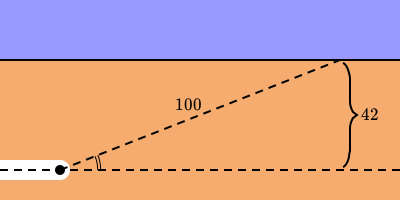
\includegraphics[width=0.5\textwidth]{../images/bugs.png}
    \end{center}
    \caption{Vista transversal del recorrido de Bugs.}
    \label{fig:bugs}
\end{figure}
\textbf{¿Cuál es el ángulo de elevación, en grados, del ascenso de Bugs?}\\
\textit{Redondea tu respuesta final a la décima más cercana.}